\documentclass[aspectratio=169,11pt]{beamer}

\usetheme{default}
\usecolortheme{default}
\setbeamertemplate{navigation symbols}{}
\setbeamertemplate{footline}{}
\setbeamertemplate{frametitle}[default][left]

% Colors
\definecolor{brand}{RGB}{28,90,168}
\definecolor{accent}{RGB}{16,185,129}
\definecolor{ink}{RGB}{26,26,26}
\definecolor{muted}{RGB}{107,114,128}
\definecolor{bg}{RGB}{255,255,255}
\definecolor{lightgray}{RGB}{243,244,246}
\definecolor{redtext}{RGB}{185,28,28}

\setbeamercolor{frametitle}{fg=ink}
\setbeamercolor{normal text}{fg=ink,bg=bg}
\setbeamercolor{itemize item}{fg=brand}
\setbeamercolor{itemize subitem}{fg=muted}

% Fonts
\usepackage[T1]{fontenc}
\usepackage{helvet}
\renewcommand{\familydefault}{\sfdefault}
\setbeamerfont{frametitle}{size=\Large,series=\bfseries}

% Packages
\usepackage{tikz}
\usepackage{booktabs}

% Helpers
\newcommand{\pill}[1]{%
  \tikz[baseline=(t.base)]{\node[fill=brand!10,text=brand,rounded corners=3pt,inner sep=3pt,font=\footnotesize\bfseries](t){#1};}%
}
\newcommand{\greenpill}[1]{%
  \tikz[baseline=(t.base)]{\node[fill=accent!15,text=accent!80!black,rounded corners=3pt,inner sep=3pt,font=\footnotesize\bfseries](t){#1};}%
}
\newcommand{\chmark}{{\color{accent!80!black}\checkmark}\;}

% -----------------------------------------------------------
\begin{document}

% ======================== SLIDE 1 ========================
\begin{frame}
\vfill
\begin{center}
  {\color{brand}\fontsize{40}{44}\selectfont\bfseries CaseBridge}\\[10pt]
  {\color{ink}\large One interview. Five applications. Zero data leaks.}\\[24pt]
  \pill{CPP AI Hackathon 2026}\quad\pill{Category 5}\quad\pill{SDGs 1 $\cdot$ 3 $\cdot$ 10 $\cdot$ 11}\\[18pt]
  {\color{brand}\normalsize\bfseries casebridge.live}\\[10pt]
  {\color{muted}\small Team Lebroncos}
\end{center}
\vfill
\end{frame}

% ======================== SLIDE 2 ========================
\begin{frame}{The Problem}
\vspace{4pt}
\begin{center}
  {\color{brand}\fontsize{44}{48}\selectfont\bfseries 60--70\%}\\[4pt]
  {\color{muted}\normalsize of a social worker's time goes to paperwork}
\end{center}
\vspace{10pt}
\begin{columns}[T]
  \begin{column}{0.46\textwidth}
    {\small\textbf{What they do now:}}
    \begin{itemize}\small
      \item 45-min intake per client
      \item Check 5+ program eligibilities manually
      \item Fill each application form by hand
      \item Repeat 15--20 times per day
    \end{itemize}
  \end{column}
  \begin{column}{0.46\textwidth}
    {\small\textbf{\color{brand}What it costs:}}
    \begin{itemize}\small
      \item 15+ hours/week on admin alone
      \item Eligible families miss programs
      \item Clients wait weeks for benefits
      \item 40\% annual caseworker turnover
    \end{itemize}
  \end{column}
\end{columns}
\end{frame}

% ======================== SLIDE 3 ========================
\begin{frame}{CaseBridge: AI Co-Pilot for Social Workers}
\vspace{2pt}
\begin{center}
  {\color{muted}\small One conversation in \;\;$\longrightarrow$\;\; Five filled applications out}
\end{center}
\vspace{6pt}
\begin{columns}[T]
  \begin{column}{0.44\textwidth}
    {\small\textbf{Six agents, one pipeline:}}\\[6pt]
    {\footnotesize
    \begin{tabular}{@{}ll@{}}
      \greenpill{Intake}      & Conversational interview \\[3pt]
      \greenpill{Profile}     & Normalize \& validate \\[3pt]
      \greenpill{Risk}        & Red/amber safety flags \\[3pt]
      \greenpill{Research}    & Match programs \\[3pt]
      \greenpill{Eligibility} & Deterministic rules \\[3pt]
      \greenpill{Packet}      & Pre-filled PDFs \\
    \end{tabular}}
  \end{column}
  \begin{column}{0.50\textwidth}
    {\small\textbf{What makes it different:}}\\[6pt]
    {\footnotesize
    \textbf{100\% local AI} --- Gemma 4 on your GPU\\
    {\color{muted}No data leaves the machine. Ever.}\\[5pt]
    \textbf{140+ languages} --- auto-detected\\
    {\color{muted}Type in Spanish, Vietnamese, Farsi\ldots}\\[5pt]
    \textbf{Deterministic eligibility}\\
    {\color{muted}Auditable rules, not LLM guesses}\\[5pt]
    \textbf{Real application PDFs}\\
    {\color{muted}AcroForm templates for 5 CA programs}}
  \end{column}
\end{columns}
\end{frame}

% ======================== SLIDE 4 ========================
\begin{frame}{Live Demo}
\vspace{6pt}
\begin{center}
  {\color{brand}\Large\bfseries casebridge.live}
\end{center}
\vspace{10pt}
\begin{center}

\begin{tikzpicture}
  \node[fill=lightgray,rounded corners=6pt,inner sep=10pt] {
    \footnotesize
    \pill{New Case}$\;\to\;$%
    \pill{Intake}$\;\to\;$%
    \pill{Profile}$\;\to\;$%
    \pill{Eligibility}$\;\to\;$%
    \pill{Packet}%
  };
\end{tikzpicture}
\end{center}
\vspace{12pt}
\begin{columns}[T]
  \begin{column}{0.30\textwidth}
    \centering
    {\color{brand}\large$\diamondsuit$}\\[2pt]
    {\small\textbf{Intake}}\\[2pt]
    {\color{muted}\scriptsize Empathetic, one question\\at a time, any language}
  \end{column}
  \begin{column}{0.30\textwidth}
    \centering
    {\color{accent!80!black}\large\checkmark}\\[2pt]
    {\small\textbf{Eligibility}}\\[2pt]
    {\color{muted}\scriptsize 5 programs, deterministic\\rules, clear reasons}
  \end{column}
  \begin{column}{0.30\textwidth}
    \centering
    {\color{brand}\large$\Downarrow$}\\[2pt]
    {\small\textbf{Packet}}\\[2pt]
    {\color{muted}\scriptsize Pre-filled PDFs, caseworker\\reviews before submission}
  \end{column}
\end{columns}
\end{frame}

% ======================== SLIDE 5 ========================
\begin{frame}{Privacy by Architecture}
\vspace{4pt}
\begin{center}
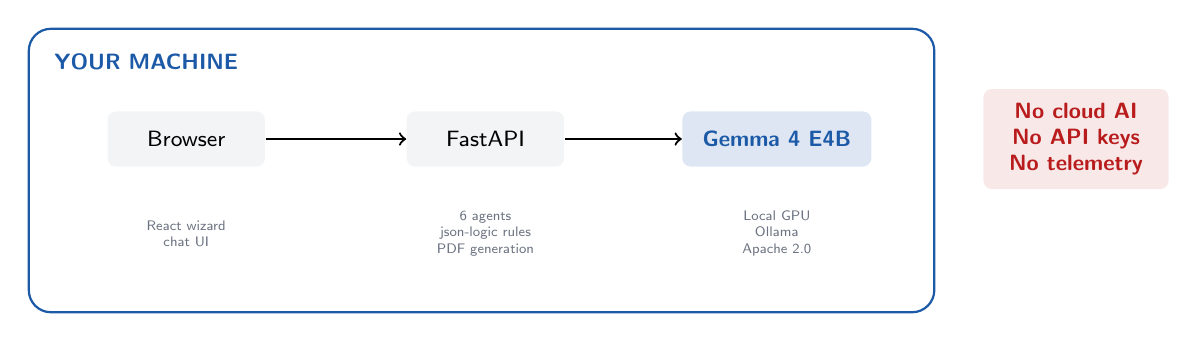
\begin{tikzpicture}
  \draw[rounded corners=8pt, thick, brand] (0,0) rectangle (11.5,3.6);
  \node[anchor=north west, font=\footnotesize\bfseries, color=brand] at (0.2,3.4) {YOUR MACHINE};
  \node[fill=lightgray, rounded corners=3pt, minimum width=2cm, minimum height=0.7cm, font=\footnotesize] (b) at (2, 2.2) {Browser};
  \node[fill=lightgray, rounded corners=3pt, minimum width=2cm, minimum height=0.7cm, font=\footnotesize] (a) at (5.8, 2.2) {FastAPI};
  \node[fill=brand!15, rounded corners=3pt, minimum width=2.4cm, minimum height=0.7cm, font=\footnotesize\bfseries, text=brand] (g) at (9.5, 2.2) {Gemma 4 E4B};
  \draw[->, thick] (b) -- (a);
  \draw[->, thick] (a) -- (g);
  \node[font=\tiny, color=muted, text width=2cm, align=center] at (2, 1.0) {React wizard\\chat UI};
  \node[font=\tiny, color=muted, text width=2cm, align=center] at (5.8, 1.0) {6 agents\\json-logic rules\\PDF generation};
  \node[font=\tiny, color=muted, text width=2cm, align=center] at (9.5, 1.0) {Local GPU\\Ollama\\Apache 2.0};
  % Red block outside
  \node[fill=redtext!10, rounded corners=3pt, text=redtext, font=\footnotesize\bfseries, text width=2cm, align=center, inner sep=5pt] at (13.3, 2.2) {No cloud AI\\No API keys\\No telemetry};
\end{tikzpicture}
\end{center}
\vspace{6pt}
\begin{columns}[T]
  \begin{column}{0.46\textwidth}
    {\footnotesize
    \chmark Data in memory only --- no database\\
    \chmark Destroyed on restart --- no persistence\\
    \chmark CSP header blocks external AI calls\\
    \chmark Zero cloud AI imports in codebase}
  \end{column}
  \begin{column}{0.46\textwidth}
    {\footnotesize
    \chmark Works fully offline (verified)\\
    \chmark HIPAA-ready architecture by default\\
    \chmark Eligibility is deterministic \& auditable\\
    \chmark Caseworker reviews before submission}
  \end{column}
\end{columns}
\end{frame}

% ======================== SLIDE 6 ========================
\begin{frame}{Impact}
\vspace{8pt}
\begin{center}
  \begin{minipage}{0.22\textwidth}\centering
    {\color{brand}\fontsize{26}{30}\selectfont\bfseries 4:32}\\[2pt]
    {\color{muted}\footnotesize avg session}
  \end{minipage}\hfill
  \begin{minipage}{0.22\textwidth}\centering
    {\color{brand}\fontsize{26}{30}\selectfont\bfseries 45m}\\[2pt]
    {\color{muted}\footnotesize manual avg}
  \end{minipage}\hfill
  \begin{minipage}{0.22\textwidth}\centering
    {\color{brand}\fontsize{26}{30}\selectfont\bfseries 90\%}\\[2pt]
    {\color{muted}\footnotesize time saved}
  \end{minipage}\hfill
  \begin{minipage}{0.22\textwidth}\centering
    {\color{brand}\fontsize{26}{30}\selectfont\bfseries 5}\\[2pt]
    {\color{muted}\footnotesize programs}
  \end{minipage}
\end{center}
\vspace{14pt}
\begin{center}
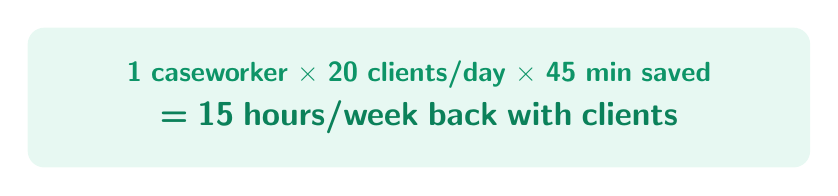
\begin{tikzpicture}
  \node[fill=accent!10,rounded corners=6pt,inner sep=12pt,text width=0.75\textwidth,align=center] {
    {\color{accent!80!black}\normalsize\bfseries 1 caseworker $\times$ 20 clients/day $\times$ 45 min saved}\\[4pt]
    {\color{accent!70!black}\large\bfseries = 15 hours/week back with clients}
  };
\end{tikzpicture}
\end{center}
\vspace{10pt}
\begin{center}
  \pill{SDG 1} {\footnotesize Benefits access}\;\;
  \pill{SDG 3} {\footnotesize Healthcare}\;\;
  \pill{SDG 10} {\footnotesize 140+ languages}\;\;
  \pill{SDG 11} {\footnotesize Local resources}
\end{center}
\end{frame}

% ======================== SLIDE 7 ========================
\begin{frame}{Tech Stack \& Roadmap}
\vspace{4pt}
\begin{columns}[T]
  \begin{column}{0.44\textwidth}
    {\small\textbf{Built with:}}\\[4pt]
    {\footnotesize
    \begin{tabular}{@{}ll@{}}
      \textbf{AI}      & Gemma 4 E4B / Ollama \\
      \textbf{Front}   & React 19, Vite, Tailwind \\
      \textbf{Back}    & FastAPI, Pydantic \\
      \textbf{Rules}   & json-logic (deterministic) \\
      \textbf{PDF}     & pdf-lib, reportlab, pypdf \\
      \textbf{Deploy}  & SSH tunnel to VPS \\
    \end{tabular}}
    \vspace{8pt}

    {\small\textbf{Accuracy:}}\\[4pt]
    {\footnotesize
    \chmark Eligibility: \textbf{deterministic}, 0\% variance\\
    \chmark Extraction: LLM + \textbf{caseworker review}\\
    \chmark Rules from public FPL schedules\\
    \chmark Git-versioned, auditable JSON}
  \end{column}
  \begin{column}{0.48\textwidth}
    {\small\textbf{Deployment roadmap:}}\\[4pt]
    {\footnotesize
    \begin{description}\setlength{\itemsep}{4pt}
      \item[\color{brand}Phase 1] Pilot: 1 LA County DSS office\\
        {\color{muted}5 caseworkers, 3 months}
      \item[\color{brand}Phase 2] Scale: 5 California counties\\
        {\color{muted}State-specific rule sets}
      \item[\color{brand}Phase 3] CDSS state-wide partnership\\
        {\color{muted}BAA-covered infrastructure}
      \item[\color{brand}Phase 4] Open-source rules engine\\
        {\color{muted}Other states bring their own rules}
    \end{description}}
  \end{column}
\end{columns}
\vspace{6pt}
\begin{center}
  {\color{brand}\normalsize\bfseries casebridge.live}\quad{\color{muted}\footnotesize github.com/Ryan-Simpson/CaseBridge}
\end{center}
\end{frame}

\end{document}
